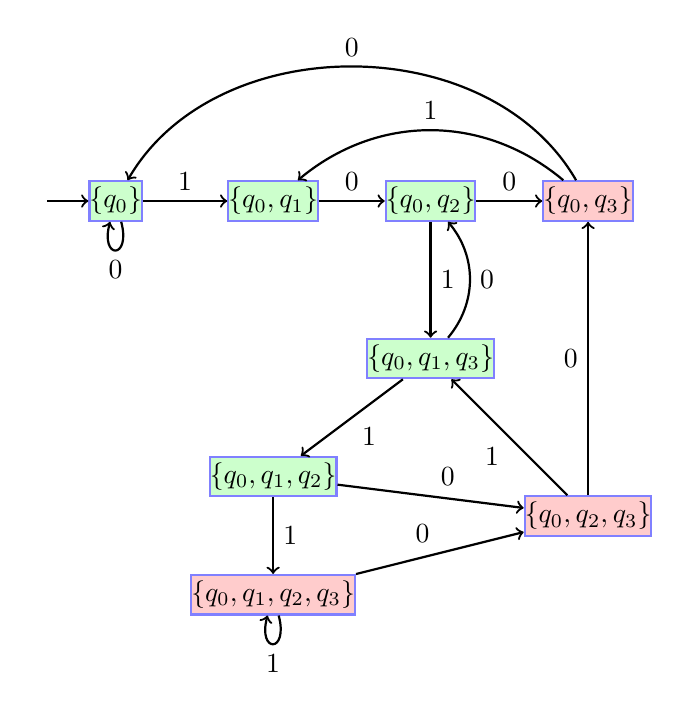
\begin{tikzpicture}



	\node 	(e0)		at	(-1,0) 	[rectangle, thick]{};

	\node 	(e1)		at	(0,0) 	[rectangle, thick, draw=blue!50,fill=green!20,inner sep=0pt,minimum size=.5cm]{$\{q_0\}$};

	\node 	(e2)		at	(2,0) 	[rectangle, thick, draw=blue!50,fill=green!20,inner sep=0pt,minimum size=.5cm]{$\{q_0,q_1\}$};


	\node 	(e3)		at	(4,0) 	[rectangle, thick, draw=blue!50,fill=green!20,inner sep=0pt,minimum size=.5cm]{$\{q_0,q_2\}$};



	\node 	(e4)		at	(6,0) 	[rectangle, thick, draw=blue!50,fill=red!20,inner sep=0pt,minimum size=.5cm]{$\{q_0,q_3\}$};


	\node 	(e5)		at	(4,-2) 	[rectangle, thick, draw=blue!50,fill=green!20,inner sep=0pt,minimum size=.5cm]{$\{q_0,q_1,q_3\}$};

	\node 	(e6)		at	(2,-3.5) 	[rectangle, thick, draw=blue!50,fill=green!20,inner sep=0pt,minimum size=.5cm]{$\{q_0,q_1,q_2\}$};

	\node 	(e7)		at	(2,-5) 	[rectangle, thick, draw=blue!50,fill=red!20,inner sep=0pt,minimum size=.5cm]{$\{q_0,q_1,q_2,q_3\}$};

	\node 	(e8)		at	(6,-4) 	[rectangle, thick, draw=blue!50,fill=red!20,inner sep=0pt,minimum size=.5cm]{$\{q_0,q_2,q_3\}$};

	\draw[->, thick]	(e0)	to	node[auto]{}	(e1);
	\draw[->, thick]	(e1)	to	node[auto]{$1$}	(e2);
	\draw[->, thick]	(e2)	to	node[auto]{$0$}	(e3);
	\draw[->, thick]	(e3)	to	node[auto]{$0$}	(e4);

	\draw[->, thick]	(e3)	to	node[auto]{$1$}	(e5);
	\draw[->, thick]	(e5)	to	node[auto]{$1$}	(e6);
	\draw[->, thick]	(e6)	to	node[auto]{$1$}	(e7);
	\draw[->, thick]	(e6)	to	node[auto]{$0$}	(e8);
	\draw[->, thick]	(e8)	to	node[auto]{$1$}	(e5);
	\draw[->, thick]	(e8)	to	node[auto]{$0$}	(e4);
	\draw[->, thick]	(e7)	to	node[auto]{$0$}	(e8);


	\draw[->, thick,bend right=40]	(e5)	to	node[auto,swap]{$0$}	(e3);
	\draw[->, thick,bend right=40]	(e4)	to	node[auto,swap]{$1$}	(e2);
	\draw[->, thick,bend right=60]	(e4)	to	node[auto,swap]{$0$}	(e1);

	\draw[->, thick,loop below]	(e1)	to	node[auto]{$0$}	(e1);
	\draw[->, thick,loop below]	(e7)	to	node[auto]{$1$}	(e7);

%	\draw[->, thick,bend right=30]	(e5)	to	node[auto,swap]{$b$}	(e2);


\end{tikzpicture}

